    \documentclass{article}
\usepackage[utf8]{inputenc}
\usepackage{amsmath}
\usepackage{graphicx}
\usepackage{setspace}
\usepackage{mathtools}
\usepackage{subfig}
\usepackage{caption}
\usepackage{placeins}
\usepackage{multirow}
\usepackage{longtable}
\usepackage{indentfirst}
\usepackage[obeyspaces]{url}
\usepackage{ragged2e}
\usepackage{float}
\usepackage[bottom]{footmisc}


%Paragraph jumps and indentation
\setlength{\parskip}{1.6em}
\setlength{\parindent}{1.25cm}
%Border
\usepackage[left=1in, right=1in, top=1in, bottom=1in]{geometry}



\begin{document}

\begin{center}
    \par{\huge \textbf{The Effect of Temperature on the Elasticity of a Material}}
\end{center}


\section{Introduction}

\urlstyle{same}

\par{The Young's Modulus is a fundamental property of the material and is, thus, unaffected by the dimensions of the object and only affected by properties that affect the atoms of the material.\footnote{\RaggedRight \url{Stoeboe, Tom. Young’s Modulus. https://depts.washington.edu/matseed/mse_resources/Webpage/Biomaterials/young\%27s_modulus.htm. Accessed 1 Aug. 2021.}}
 Properties that promote dislocation of the particles of the material on the atomic scale would reduce the elasticity of the material. It was this intrinsic nature of Young's Modulus that made me want to better understand the relationship between elasticity and temperature. Elasticity has many uses and planning for the effect of temperature on elasticity would be an important step in determining the use of a material. As the son of an engineer, I noticed that my father takes the effect of temperature on materials seriously when designing transformers and prioritises more elastic materials for hotter regions. He does this to reduce power losses through copper wires and increase the power availability in hot regions. I want to verify his diligence as this would provide me insight into how the elasticity of a material changes and how to mitigate these changes.}

\subsection{Background Information}

\subsubsection{Elasticity}

\par{The elasticity of a material is an important property with many applications in our lives, from stretching our limbs to designing safe buildings. The term refers to the ability of a material to return to its original shape and size after a deforming force has been removed\footnotemark. An elastic material is one that can return to its original state after the deforming state has been removed. A plastic material is one that remains deformed despite the removal of the deforming force \newline}

\footnotetext{Young, Hugh D, Roger A. Freedman, A L. Ford, Mark W. Zemansky, and Francis W. Sears. Sears and Zemansky's University Physics. San Francisco [Calif.: Pearson Addison-Wesley, 2008. Print.}

\subsubsection{Young's Modulus}

\par{Alternatively\footnote{Sadd, Martin H. Elasticity: Theory, Applications, and Numerics. 2010.
}, the elasticity of a material may be described as the ratio of stress (the force applied on an object causing its deformation) to strain (a measure of the deformation resulting from stress): its elastic modulus. The lesser the strain produced from a stress relative to a material, the more elastic the material. This can be modelled by the following equations: }


\begin{equation}
    \text{Elastic~Modulus} = \frac{\text{Stress}}{\text{Strain}}
\end{equation} 

\par{A familiar elastic behaviour is that of stretching a wire or a rod at both ends. Figure 1 depicts a box of uniform length $L_0$ and cross-sectional area A.}

\begin{center}
     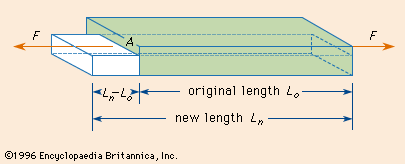
\includegraphics[scale=0.85]{bar.png}
   \par{Figure 1: Bar with uniform length and area being stretched\protect\footnotemark} 
\end{center}

\footnotetext{Britannica, The Editors of Encyclopaedia. "Young's modulus". Encyclopedia Britannica, 3 Jul. 2019, https://www.britannica.com/science/Youngs-modulus.}


\par{By applying a deforming force, $F_{\bot}$ on both ends in opposite directions (so that the object remains stationary), the object will be in tension, i.e. it would be experiencing a force along its length. This force is being is acting perpendicular to the cross-sectional area and the quantity, deforming force acting per unit cross-sectional area is tensile stress.}

\begin{equation}
    \text{Tensile~Stress} = \frac{F_{\bot}}{A}
    \end{equation} 

\par{Under this tension, the body will stretch to a length $L_n$ = $\Delta L$ + $L_0$. This elongation $\Delta$L is experienced throughout the body and not just the ends. The ratio of the elongation to the initial length is Tensile Strain}

\begin{equation}
    \text{Tensile~Strain} = \frac{\Delta L}{L_0}
\end{equation} 

\par{Now that the Tensile Stress and Strain have been identified, the Elastic Modulus of a material can be restated in terms of Tensile Stress and Strain. Substituting equation 2 and 3 into equation 1, we get the Young's Modulus Y of a material, a constant that measures the tensile stiffness of a material.}

\begin{equation}
    \text{Y} = \frac{\text{Tensile~Stress}}{\text{Tensile~Strain}} = \frac{\frac{F_{\bot}}{A}}{\frac{\Delta L}{L_0}}
\end{equation} 

\par{Where $F_{\bot}$ is the deforming force, A is the cross-sectional area of the material, $\Delta L$ is the change in length of the material due to the deforming force, and $L_0$ is the initial length of the material \newline

}
\section{Design}

\subsection{Research Question}

\par{How does the temperature of a material relate to its elasticity?}

\subsection{Hypothesis}

\par{An increase in temperature (T) would reduce the Young's Modulus (Y) of a material and thus result in it becoming less elastic over a higher range of temperatures. This is because the increased temperature would result in a greater number of vibrations between atoms, which would decrease the force between atoms and increase atomic distance. If Y is plotted against T and all other variables are kept constant, a linear graph with a steep, negative slope would be obtained.}
\vspace{-0.5cm}
\subsection{Variables}

\begin{spacing}{2}
    \par{\vspace{-0.5cm} \hspace{-1.4cm}
    \textbf{A. Independent Variable:} Temperature of the wire (T) \newline
    \textbf{B. Dependent Variable:} Young's Modulus of the wire (Y) \newline
    \textbf{C. Control Variables:} \newline
   \hspace*{1cm} \textbf{I. Material} \newline}
\end{spacing}

\hfill\begin{minipage}{\dimexpr\textwidth-1cm}
\vspace{-1cm}
\par{\textbf{a) Reason:} As Young's Modulus of a material is a property intrinsic to a material, different materials (even if the material has a small impurity) would have different Young's Moduli. \newline
\textbf{b) Method:} Throughout the experiment, I used only one type of material: a copper wire. This was to ensure that there was no inconsistencies due to material. Additionally, the dimensions of the material were kept constant at a of 0.00128m and a length of 1.7m. \newline}
\xdef\tpd{\the\prevdepth}
\end{minipage}

\begin{spacing}{2}
 \textbf{II. Pressure}
\end{spacing}

\hfill\begin{minipage}{\dimexpr\textwidth-1cm}
\par{\textbf{a) Reason:} Increasing pressure would reduce the dislocation of particles of the material and would,
thus, increase the value of the Young’s Modulus.6
 \footnotemark \newline
\textbf{b) Method:} I kept the copper wires in a box of uniform length and area of pressure 1 atm.\newline}
\xdef\tpd{\the\prevdepth}
\end{minipage}
\footnotetext{Li, Wb., Li, K., Fan, Kq. et al. Temperature and Pressure Dependences of the Elastic Properties of Tantalum Single Crystals Under $<100>$ Tensile Loading: A Molecular Dynamics Study. Nanoscale Res Lett 13, 118 (2018). https://doi.org/10.1186/s11671-018-2526-1}

\begin{spacing}{2}
    \textbf{III. Ambient Temperature}
\end{spacing}

\hfill\begin{minipage}{\dimexpr\textwidth-1cm}
\par{\textbf{a) Reason:} Different ambient temperatures may result in the wire experiencing a lower temperature than is reported by the thermometer due to cooling. Additionally, it may also result in fatiguing because of cooling the wire after heating it to a high temperature which would reduce elasticity. \newline
\textbf{b) Method:} Throughout the experiment, I conducted the experiment in a single room at 30°C. The copper wire was insulated by a metal box. Additionally, I used different wires with the same dimensions at different temperatures to mitigate the effects of fatiguing.\newline}
\xdef\tpd{\the\prevdepth}
\end{minipage}

\begin{spacing}{2}
    \textbf{III. Stress}
\end{spacing}

\hfill\begin{minipage}{\dimexpr\textwidth-1cm}
\par{\textbf{a) Reason:} Subjecting a material to a large number of stresses would result in it remaining deformed even within it's elastic limit \newline
\textbf{b) Method:} Throughout the experiment, I changed the copper wire.\newline}
\xdef\tpd{\the\prevdepth}
\end{minipage}

\vspace{-1cm}
\subsection{Apparatus}

\begin{enumerate}
    \item Safety Goggles
    \item Oven
    \item Digital Thermometer
    \item Ruler
    \item Load/Weights 
    \item G-Clamp
    \item Pulley
    \item Wire
    \item Micrometer
\end{enumerate}
\vspace{-0.5cm}
\subsubsection{Experimental Set-Up}
\begin{figure}[!h]
    \centering
    \caption{Schematic of Experimental Set-up}
    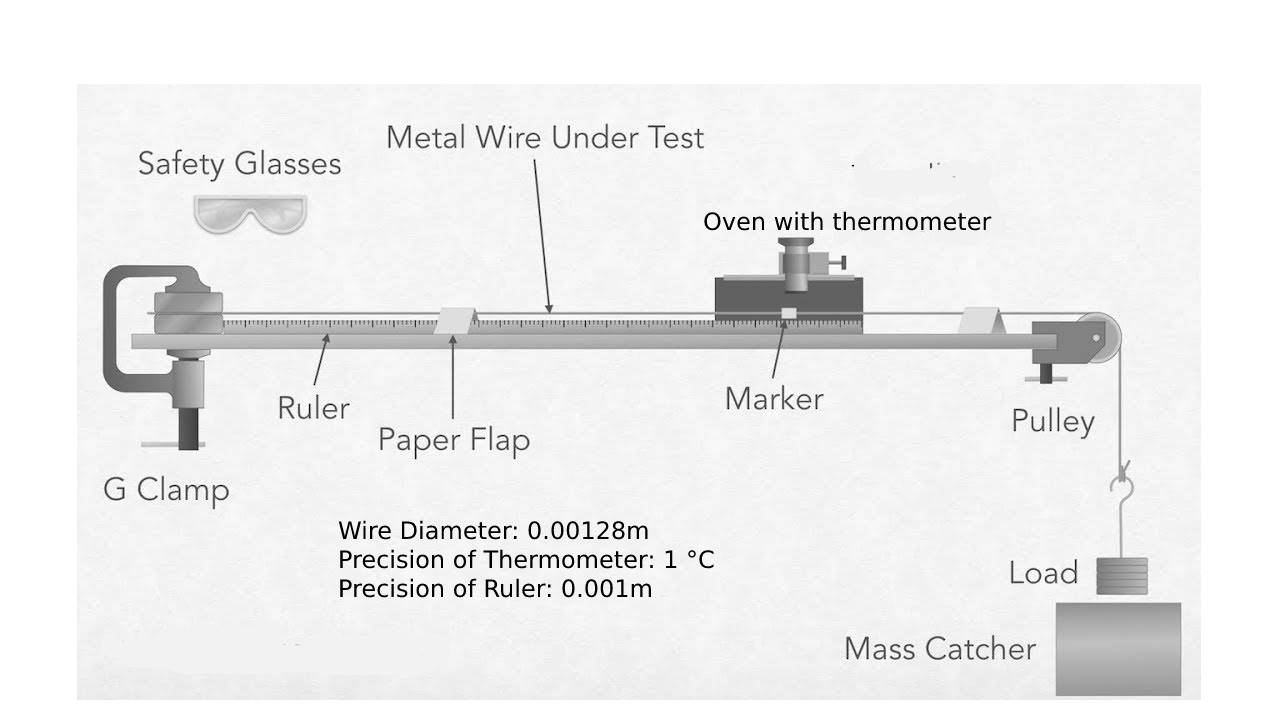
\includegraphics[width=12cm]{imageonline-co-blackandwhiteimage (1).jpg} 
\end{figure}
\FloatBarrier

\subsection{Procedure}

\subsubsection{Safety Precautions}

\par{I wrapped one end of the wire firmly around a block that was clamped down on the table. This was done to prevent the wire from slipping and flicking the face. Additionally, to prevent the wire from striking my face, a paper card was placed above the wire, a glass cover was placed on top of the oven where the wire was placed and safety goggles were worn. A mass catcher was placed below the load to dampen shocks. I ensured that my body parts were away from the mass. There were no ethical or environmental considerations for this experiment. The copper was re-used to prevent wastage.}
\vspace{-0.5cm}
\subsubsection{Methodology}

\begin{enumerate}
    \item First, I wrapped one end of the wire firmly around a block that was clamped down on the table. 
    \item Next, I strung the other end of the wire around the pulley and wrapped around the load.
    \item I stuck a piece of tape onto the wire at the 50cm mark to measure the elongation $\Delta L$. I increased the temperature of the oven to 28°C
    \item I loaded a mass (M) of 8 kg onto the load and measured the extension.
    \item To the 8kg mass, I loaded a 6kg mass and measured the extension.
    \item To the 14kg mass, I loaded a 6kg mass and measured the extension
    \item To the 20kg mass, I loaded a 6kg mass and measured the extension
    \item To the 26kg mass, I loaded a 6kg mass and measured the extension
    \item I repeated steps 4-9 5 times
    \item I repeated steps 1-10 at 33°C
    \item I repeated steps 1-10 at 39°C
    \item I repeated steps 1-10 at 43°C
            \begin{itemize}
            \item At 32kg, the wire reached its yield point.
        \end{itemize}
    \item I repeated steps 1-10 at 46°C
                \begin{itemize}
            \item At 26kg, the wire reached its yield point.
        \end{itemize}
    \item I repeated steps 1-10 at 49°C
                \begin{itemize}
            \item At 27kg, the wire reached its yield point.
        \end{itemize}
\end{enumerate}
\vspace{-0.75cm}
\par{Further readings were not taken as the wire was fatigued at low loads.}
\vspace{-0.5cm}
\subsection{Data Collection}
\vspace{-0.5cm}
\begin{longtable}[c]{|l|l|l|l|l|l|}
\caption{Extension of wire at 28°C}
\label{tab:my-table}\\
\hline
\multicolumn{6}{|c|}{\textbf{Temperature of Wire (°C) 28°C ± 0.1°C}} \\ \hline
\endfirsthead
%
\multicolumn{6}{c}%
{{\bfseries Table \thetable\ continued from previous page}} \\
\hline
\multicolumn{6}{|c|}{\textbf{Temperature of Wire (°C) 28°C ± 0.1°C}} \\ \hline
\endhead
%
\multicolumn{1}{|c|}{\multirow{2}{*}{\textbf{Mass of Load (kg)}}} &
  \multicolumn{5}{c|}{\textbf{Extension of Wire ($\boldsymbol{10^{-3}}$ m) ± 0.001m}} \\ \cline{2-6} 
\multicolumn{1}{|c|}{} &
  \textbf{Trial 1} &
  \multicolumn{1}{c|}{\textbf{Trial 2}} &
  \multicolumn{1}{c|}{\textbf{Trial 3}} &
  \textbf{Trial 4} &
  \textbf{Trial 5} \\ \hline
8.00         & 2.0         & 2.0         & 3.0        & 3.0       & 2.0         \\ \hline
14.00        & 6.0         & 5.0         & 5.0        & 5.0       & 5.5       \\ \hline
20.00        & 25.0        & 26.0        & 24.0       & 24.0        & 26.0        \\ \hline
26.00        & 59.0        & 60.0        & 58.0       & 58.0        & 58.0        \\ \hline
32.00        & 69.0        & 70.0        & 70.0       & 69.0        & 70.0        \\ \hline
\end{longtable}

\begin{longtable}[c]{|l|l|l|l|l|l|}
\caption{Extension of wire at 33°C}
\label{tab:my-table}\\
\hline
\multicolumn{6}{|c|}{\textbf{Temperature of Wire (°C) 33°C ± 0.1°C}} \\ \hline
\endfirsthead
%
\multicolumn{6}{c}%
{{\bfseries Table \thetable\ continued from previous page}} \\
\hline
\multicolumn{6}{|c|}{\textbf{Temperature of Wire (°C) 28°C ± 0.1°C}} \\ \hline
\endhead
%
\multicolumn{1}{|c|}{\multirow{2}{*}{\textbf{Mass of Load (kg)}}} &
  \multicolumn{5}{c|}{\textbf{Extension of Wire ($\boldsymbol{10^{-3}}$ m) ± 0.001m}} \\ \cline{2-6} 
\multicolumn{1}{|c|}{} &
  \textbf{Trial 1} &
  \multicolumn{1}{c|}{\textbf{Trial 2}} &
  \multicolumn{1}{c|}{\textbf{Trial 3}} &
  \textbf{Trial 4} &
  \textbf{Trial 5} \\ \hline
8.00         & 6.0         & 5.0         & 6.0         & 5.5       & 6.0        \\ \hline
14.00        & 10.0        & 11.0        & 9.0         & 9.0         & 11.0       \\ \hline
20.00        & 28.0        & 29.0        & 27.0        & 29.0        & 27.0       \\ \hline
26.00        & 40.0        & 39.0        & 41.0        & 39.0        & 41.0       \\ \hline
32.00        & 70.0        & 71.0        & 69.0        & 69.0        & 71.0       \\ \hline
\end{longtable}

\begin{longtable}[c]{|l|l|l|l|l|l|}
\caption{Extension of wire at 39°C}
\label{tab:my-table}\\
\hline
\multicolumn{6}{|c|}{\textbf{Temperature of Wire (°C) 39°C ± 0.1°C}} \\ \hline
\endfirsthead
%
\multicolumn{6}{c}%
{{\bfseries Table \thetable\ continued from previous page}} \\
\hline
\multicolumn{6}{|c|}{\textbf{Temperature of Wire (°C) 39°C ± 0.1°C}} \\ \hline
\endhead
%
\multicolumn{1}{|c|}{\multirow{2}{*}{\textbf{Mass of Load (kg)}}} &
  \multicolumn{5}{c|}{\textbf{Extension of Wire ($\boldsymbol{10^{-3}}$ m) ± 0.001m}} \\ \cline{2-6} 
\multicolumn{1}{|c|}{} &
  \textbf{Trial 1} &
  \multicolumn{1}{c|}{\textbf{Trial 2}} &
  \multicolumn{1}{c|}{\textbf{Trial 3}} &
  \textbf{Trial 4} &
  \textbf{Trial 5} \\ \hline
8.00        & 5.0         & 7.0         & 8.0         & 5.5        & 8.0        \\ \hline
14.00       & 9.0         & 12.0        & 11.0        & 10.0       & 12.0       \\ \hline
20.00       & 27.0        & 29.0        & 29.0        & 28.0         & 27.0       \\ \hline
26.00       & 75.0        & 74.0        & 77.0        & 76.0         & 75.0       \\ \hline
32.00       & 120.0       & 121.0       & 118.0       & 120.0        & 119.0      \\ \hline
\end{longtable}

\begin{longtable}[c]{|l|l|l|l|l|l|}
\caption{Extension of wire at 43°C}
\label{tab:my-table}\\
\hline
\multicolumn{6}{|c|}{\textbf{Temperature of Wire (°C) 43°C ± 0.1°C}} \\ \hline
\endfirsthead
%
\multicolumn{6}{c}%
{{\bfseries Table \thetable\ continued from previous page}} \\
\hline
\multicolumn{6}{|c|}{\textbf{Temperature of Wire (°C) 43°C ± 0.1°C}} \\ \hline
\endhead
%
\multicolumn{1}{|c|}{\multirow{2}{*}{\textbf{Mass of Load (kg)}}} &
  \multicolumn{5}{c|}{\textbf{Extension of Wire ($\boldsymbol{10^{-3}}$ m) ± 0.001m}} \\ \cline{2-6} 
\multicolumn{1}{|c|}{} &
  \textbf{Trial 1} &
  \multicolumn{1}{c|}{\textbf{Trial 2}} &
  \multicolumn{1}{c|}{\textbf{Trial 3}} &
  \textbf{Trial 4} &
  \textbf{Trial 5} \\ \hline
8.00        & 11.0        & 12.0        & 12.0        & 11.0       & 12.0       \\ \hline
14.00       & 12.0         & 11.0        & 9.0        & 12.0       & 10.0       \\ \hline
20.00       & 27.0        & 30.0        & 29.0        & 28.0         & 29.0       \\ \hline
26.00       & 77.0        & 77.0        & 77.0        & 77.0         & 77.0       \\ \hline
32.00       & 124.0       & 125.0       & 126.0       & 126.0    & 124.0      \\ \hline
\end{longtable}

\begin{longtable}[c]{|l|l|l|l|l|l|}
\caption{Extension of wire at 46°C}
\label{tab:my-table}\\
\hline
\multicolumn{6}{|c|}{\textbf{Temperature of Wire (°C) 46°C ± 0.1°C}} \\ \hline
\endfirsthead
%
\multicolumn{6}{c}%
{{\bfseries Table \thetable\ continued from previous page}} \\
\hline
\multicolumn{6}{|c|}{\textbf{Temperature of Wire (°C) 46°C ± 0.1°C}} \\ \hline
\endhead
%
\multicolumn{1}{|c|}{\multirow{2}{*}{\textbf{Mass of Load (kg)}}} &
  \multicolumn{5}{c|}{\textbf{Extension of Wire ($\boldsymbol{10^{-3}}$ m) ± 0.001m}} \\ \cline{2-6} 
\multicolumn{1}{|c|}{} &
  \textbf{Trial 1} &
  \multicolumn{1}{c|}{\textbf{Trial 2}} &
  \multicolumn{1}{c|}{\textbf{Trial 3}} &
  \textbf{Trial 4} &
  \textbf{Trial 5} \\ \hline
8.00         & 13.0         & 13.0       & 12.0        & 12.0       & 13.0        \\ \hline
14.00        & 16.0         & 17.0       & 15.0        & 17.0       & 15.0        \\ \hline
20.00        & 42.0         & 42.0       & 41.0        & 41.0       & 42.0        \\ \hline
26.00        & 100.0        & 99.0       & 101.0       & 99.0       & 101.0       \\ \hline
\end{longtable}


\begin{longtable}[c]{|l|l|l|l|l|l|}
\caption{Extension of wire at 49°C}
\label{tab:my-table}\\
\hline
\multicolumn{6}{|c|}{\textbf{Temperature of Wire (°C) 49°C ± 0.1°C}} \\ \hline
\endfirsthead
%
\multicolumn{6}{c}%
{{\bfseries Table \thetable\ continued from previous page}} \\
\hline
\multicolumn{6}{|c|}{\textbf{Temperature of Wire (°C) 49°C ± 0.1°C}} \\ \hline
\endhead
%
\multicolumn{1}{|c|}{\multirow{2}{*}{\textbf{Mass of Load (kg)}}} &
  \multicolumn{5}{c|}{\textbf{Extension of Wire ($\boldsymbol{10^{-3}}$ m) ± 0.001m}} \\ \cline{2-6} 
\multicolumn{1}{|c|}{} &
  \textbf{Trial 1} &
  \multicolumn{1}{c|}{\textbf{Trial 2}} &
  \multicolumn{1}{c|}{\textbf{Trial 3}} &
  \textbf{Trial 4} &
  \textbf{Trial 5} \\ \hline
8.00        & 14.0        & 15.0        & 16.0        & 14.0        & 16.0        \\ \hline
14.00       & 15.0        & 17.0        & 18.0        & 17.0        & 16.0        \\ \hline
20.00       & 43.0        & 40.0        & 42.0        & 41.0        & 42.0        \\ \hline
26.00       & 121.0       & 119.0       & 120.0       & 121.0       & 119.0       \\ \hline
\end{longtable}

\subsection{Data Analysis}


\par{With the collected data, the tensile stress and tensile strain was calculated for each temperature range. This was done by applying equations 2 and 3. Firstly, however, I needed to calculate the average extension $\Delta L_{\text{ave}}$ per mass per temperature. This was done by adding all 5 of the extensions measured for a specific mass at the specific temperature and then dividing the result by 5. The absolute uncertainty was calculated by calculating the range of the extensions (i.e $\frac{\Delta L_\text{max}-\Delta L_\text{min}}{2}$). After performing these results, the following data would be obtained:}

\begin{table}[h]
\caption{Average extension and uncertainty at 28 °C}
\centering
\label{tab:my-table}
\begin{tabular}{|c|c|c|}
\hline
\textbf{Mass of Load (kg)} & \textbf{$\boldsymbol{\Delta L_{ave}\; (10^{-3}\;  m)}$} & \textbf{$\boldsymbol{L_{uncertainty}\; (10^{-3}\;  m)}$} \\ \hline
8.00 & 2.4 & 0.5 \\ \hline
14.00 & 5.3 & 0.5 \\ \hline
20.00 & 25.0 & 1.0 \\ \hline
26.00 & 58.6 & 1.0 \\ \hline
32.00 & 69.6 & 0.5 \\ \hline
\end{tabular}
\end{table}

\begin{table}[h]
\caption{Average extension and uncertainty at 33 °C}
\centering
\label{tab:my-table}
\begin{tabular}{|c|c|c|}
\hline
\textbf{Mass of Load (kg)} & \textbf{$\boldsymbol{\Delta L_{ave}\; (10^{-3}\;  m)}$} & \textbf{$\boldsymbol{L_{uncertainty}\; (10^{-3}\;  m)}$} \\ \hline
8.00 & 5.7 & 0.5 \\ \hline
14.00 & 10.0 & 1.0 \\ \hline
20.00 & 28.0 & 1.0 \\ \hline
26.00 & 40.0 & 1.0 \\ \hline
32.00 & 70.0 & 1.0 \\ \hline
\end{tabular}
\end{table}

\begin{table}[h]
\centering
\caption{Average extension and uncertainty at 39 °C}
\label{tab:my-table}
\begin{tabular}{|c|c|c|}
\hline
\textbf{Mass of   Load (kg)} & \textbf{$\boldsymbol{\Delta L_{ave}\; (10^{-3}\;  m)}$} & \textbf{$\boldsymbol{L_{uncertainty}\; (10^{-3}\;  m)}$} \\ \hline
8.00 & 6.7 & 1.5 \\ \hline
14.00 & 10.8 & 1.5 \\ \hline
20.00 & 28.0 & 1.0 \\ \hline
26.00 & 75.4 & 1.5 \\ \hline
32.00 & 119.6 & 1.5 \\ \hline
\end{tabular}
\end{table}

\begin{table}[H]
\centering
\caption{Average extension and uncertainty at 43 °C}
\label{tab:my-table}
\begin{tabular}{|c|c|c|}
\hline
\textbf{Mass of Load (kg)} & \textbf{$\boldsymbol{\Delta L_{ave}\; (10^{-3}\;  m)}$} & \textbf{$\boldsymbol{L_{uncertainty}\; (10^{-3}\;  m)}$} \\ \hline
8.00 & 11.6 & 0.5 \\ \hline
14.00 & 10.8 & 1.5 \\ \hline
20.00 & 28.6 & 1.5 \\ \hline
26.00 & 77.0 & 0.0 \\ \hline
32.00 & 125.0 & 1.0 \\ \hline
\end{tabular}
\end{table}

\begin{table}[h]
\centering
\caption{Average extension and uncertainty at 46 °C}
\label{tab:my-table}
\begin{tabular}{|c|c|c|}
\hline
\textbf{Mass of Load (kg)} & \textbf{$\boldsymbol{\Delta L_{ave}\; (10^{-3}\;  m)}$} & \textbf{$\boldsymbol{L_{uncertainty}\; (10^{-3}\;  m)}$} \\ \hline
8.00 & 12.6 & 0.5 \\ \hline
14.00 & 16.0 & 1.0 \\ \hline
20.00 & 41.6 & 0.5 \\ \hline
26.00 & 100.0 & 1.0 \\ \hline
\end{tabular}
\end{table}



\begin{table}[]
\centering
\caption{Average extension and uncertainty at 49 °C}
\label{tab:my-table}
\begin{tabular}{|c|c|c|}
\hline
\textbf{Mass of   Load (kg)} & \textbf{$\boldsymbol{\Delta L_{ave}\; (10^{-3}\;  m)}$} & \textbf{$\boldsymbol{L_{uncertainty}\; (10^{-3}\;  m)}$} \\ \hline
8.00 & 15.0 & 1.0 \\ \hline
14.00 & 16.6 & 1.5 \\ \hline
20.00 & 41.6 & 1.5 \\ \hline
26.00 & 120.0 & 1.0 \\ \hline
\end{tabular}
\end{table}

\begin{table}[H]
\centering
\caption{Young's Modulus with uncertainty at 28 °C }
\label{tab:my-table}
\begin{tabular}{|c|c|c|}
\hline
\textbf{Mass of Load (kg)} & \textbf{Young's Modulus (GPa)} & \textbf{$\boldsymbol{\Delta Y}$ (GPa)} \\ \hline
8.00 & 43.2 & 9.0 \\ \hline
14.00 & 34.2 & 3.8 \\ \hline
20.00 & 10.4 & 0.6 \\ \hline
26.00 & 5.8 & 0.2 \\ \hline
32.00 & 6.0 & 0.1 \\ \hline
\end{tabular}
\end{table}

\begin{table}[H]
\centering
\caption{ Young’s Modulus with uncertainty at 33 °C}
\label{tab:my-table}
\begin{tabular}{|c|c|c|}
\hline
\textbf{Mass of   Load (kg)} & \textbf{Young's Modulus (GPa)} & \textbf{$\boldsymbol{\Delta Y}$ (GPa)} \\ \hline
8.00 & 18.2 & 1.9 \\ \hline
14.00 & 18.1 & 2.1 \\ \hline
20.00 & 9.3 & 0.5 \\ \hline
26.00 & 8.4 & 0.3 \\ \hline
32.00 & 5.9 & 0.2 \\ \hline
\end{tabular}
\end{table}

\begin{table}[H]
\centering
\caption{Young’s Modulus with uncertainty at 39 °C}
\label{tab:my-table}
\begin{tabular}{|c|c|c|}
\hline
\textbf{Mass of Load (kg)} & \textbf{Young's Modulus (GPa)} & \textbf{$\boldsymbol{\Delta Y}$ (GPa)} \\ \hline
8.00 & 15.5 & 3.7 \\ \hline
14.00 & 16.8 & 2.6 \\ \hline
20.00 & 9.3 & 0.5 \\ \hline
26.00 & 4.5 & 0.2 \\ \hline
32.00 & 3.5 & 0.1 \\ \hline
\end{tabular}
\end{table}

% Please add the following required packages to your document preamble:
% \usepackage{longtable}
% Note: It may be necessary to compile the document several times to get a multi-page table to line up properly
\begin{longtable}[c]{|c|c|c|}
\caption{Young’s Modulus with uncertainty at 43 °C}
\label{tab:my-table}\\
\hline
\textbf{Mass of Load (kg)} & \textbf{Young's Modulus (GPa)} & \textbf{$\boldsymbol{\Delta Y}$ (GPa)} \\ \hline
\endfirsthead
%
\multicolumn{3}{c}%
{{\bfseries Table \thetable\ continued from previous page}} \\
\hline
\textbf{Mass of Load (kg)} & \textbf{Young's Modulus (GPa)} & \textbf{$\boldsymbol{\Delta Y}$ (GPa)} \\ \hline
\endhead
%
8.00 & 8.9 & 0.5 \\ \hline
14.00 & 16.8 & 2.6 \\ \hline
20.00 & 9.1 & 0.6 \\ \hline
26.00 & 4.4 & 0.1 \\ \hline
32.00 & 3.3 & 0.1 \\ \hline
\end{longtable}

\begin{table}[]
\centering
\caption{Young’s Modulus with uncertainty at 46 °C}
\label{tab:my-table}
\begin{tabular}{|c|c|c|}
\hline
\textbf{Mass of Load (kg)} & \textbf{Young's Modulus (GPa)} & \textbf{$\boldsymbol{\Delta Y}$ (GPa)} \\ \hline
8.00 & 8.2 & 0.5 \\ \hline
14.00 & 11.3 & 0.9 \\ \hline
20.00 & 6.2 & 0.2 \\ \hline
26.00 & 3.4 & 0.1 \\ \hline
\end{tabular}
\end{table}

\begin{table}[]
\centering
\caption{Young’s Modulus with uncertainty at 49 °C}
\label{tab:my-table}
\begin{tabular}{|c|c|c|}
\hline
\textbf{Mass of Load (kg)} & \textbf{Young's Modulus (GPa)} & \textbf{$\boldsymbol{\Delta Y}$ (GPa)} \\ \hline
8.00 & 6.9 & 0.6 \\ \hline
14.00 & 10.9 & 1.2 \\ \hline
20.00 & 6.2 & 0.3 \\ \hline
26.00 & 2.8 & 0.1 \\ \hline
\end{tabular}
\end{table}

\begin{table}[H]
\centering
\caption{Average Young’s Modulus of the wire and uncertainty}
\label{tab:my-table}
\begin{tabular}{|c|c|c|}
\hline
\textbf{T (°C) ± 0.1°C} & $\boldsymbol{Y_{ave}\;(GPa)}$ & $\boldsymbol{\Delta Y_{ave}\;(GPa)} $ \\ \hline
28.0 & 19.9 & 18.7 \\ \hline
33.0 & 12.0 & 6.1 \\ \hline
39.0 & 9.9 & 6.7 \\ \hline
43.0 & 8.5 & 6.7 \\ \hline
46.0 & 7.3 & 4.0 \\ \hline
49.0 & 6.7 & 4.1 \\ \hline
\end{tabular}
\end{table}

\par{\Large{\textbf{Sample Calculations:}}}

\par{\vspace{0.4cm}The average extension for M = 8kg and T = 28°C was calculated as follows: \newline
\begin{equation*}
  \Delta \text{L}_{\text{ave}} &= \frac{\sum_{n=1}^{5} \Delta \text{L}}{5} = \frac{2+2+3+3+2}{5} \approx \text{2.40} \times 10^{-3}\; \text{m}\\
\end{equation*}
}

\par{The absolute uncertainty for extension at M = 8kg and T = 28°C was calculated as follows:}

\begin{equation*}
    \text{L}_{\text{uncertainty}} = \frac{\text{L}_{\text{max}} - \text{L}_{\text{min}}}{2} = \frac{3-2}{2} = 5.00 \times 10^{-4} \; \text{m} 
\end{equation*}

\par{The tensile stress for M = 8kg was calculated as follows:}

\begin{equation*}
    \text{Tensile Stress} = \frac{\text{Mass} \times 9.81}{Area} = \frac{\frac{8 \times 9.81}{1.29}}{1000} \approx 6.09 \times 10^{-2} \text{GPa}
\end{equation*}

\par{The fractional error for tensile stress at $6.09 \times 10^{-2} \text{GPa}$ was calculated as follows:}

\begin{equation*}
    \frac{\Delta \text{Tensile~Stress}}{\text{Tensile~Stress}} = \frac{\Delta \text{F}_\bot}{\text{F}_\bot} + \frac{\Delta \text{A}}{\text{A}} = \frac{\Delta \text{F}_\bot}{\text{F}_\bot} + 2 \times \frac{\Delta \text{r}}{\text{r}} = \frac{0 + 2 \times \frac{0.01}{1.28}}{1000} \approx 1.56 \times 10^{-5}\text{GPa} 
\end{equation*}

\par{The tensile strain for the extension at M = 8kg and T = 28°C:}

\begin{equation*}
    \text{Tensile~Strain} = \frac{\text{L}}{\text{L}_\text{0}} = \frac{2.4}{1700} \approx 1.41 \times 10^{-3} 
\end{equation*}

\par{The fractional error in for Tensile Strain at $1.41 \times 10^{-3}$ is:}

\begin{equation*}
    \frac{\Delta \text{Tensile~Strain}}{\text{Tensile~Strain}} = \frac{\Delta \text{L}}{\text{L}} + \frac{\Delta \text{L}_\text{i}}{\text{L}_\text{i}} = \frac{1}{1700} + \frac{0.5}{2.4} \approx 2.09 \times 10^{-1}
\end{equation*}

\par{The Young's Modulus at  Tensile Stress = $6.09 \times 10^{-2} \text{GPa}$, and Tensile Strain = $1.41 \times 10^{-3}$ is:}

\begin{equation*}
    \text{Young's~Modulus} = \frac{\text{Tensile~Stress}}{\text{Tensile~Strain}} = \frac{0.0609}{0.00141} \approx 43.2 \; \text{GPa}
\end{equation*}

\par{The uncertainty in the Young's Modulus at Young's Modulus = 43.2 Gpa is:}

\begin{equation*}
    \text{Y}_{\text{uncertainty}} = (\frac{\Delta \text{Tensile~Stress}}{\text{Tensile~Stress}} + \frac{\Delta \text{Tensile~Strain}}{\text{Tensile~Strain}}) \times \text{Y} =  (0.0000156 + 0.209) \times 43.2 \approx 9.0\text{GPa} 
\end{equation*}

\par{The average Young's Modulus at T = 28°C was calculated as follows:}

\begin{equation*}
    \text{Y}_{\text{ave}} &= \sum_{n=1}^{5} \text{Y} = \frac{43.2+34.2+10.4+5.8+6.0}{5} \approx 19.9\text{GPa} 
\end{equation*}

\par{The absolute uncertainty for the average Young's Modulus at T = 28°C was calculated as follows:}

\begin{equation*}
        \Delta \; \text{Y}_{\text{ave}} = \frac{\text{Y}_{\text{max}} - \text{Y}_{\text{min}}}{2} = \frac{43.2-5.8}{2} = 18.7 \; \text{GPa}      
\end{equation*}

\subsubsection{Graphical Analysis}

\par{With the data in table 19, $\text Y_{\text{ave}}$ can be plotted against T, which yields the following graph:}

\vspace{-0.5cm}

\begin{center}
    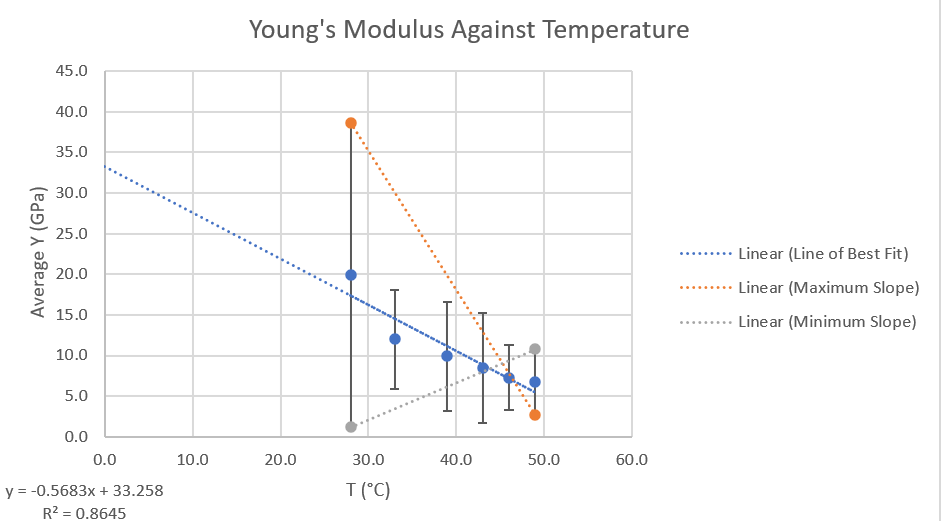
\includegraphics[scale=1]{Graph.png}
    \par{Graph 1: Graph of Young's Modulus of the wire against Temperature of the wire. Y is the Young's Modulus of the wire in GPa, while T is the temperature of the wire in °C}
\end{center}

\par{By taking any two points through which the line passes, the gradient of the line of best fit was obtained. The y intercept is observed to occur at  and thus the following equation of the graph was obtained:}

\begin{equation*}
    Y = -0.5683T + 33.258
\end{equation*}

\par{Only the error bar for the very first Young's Modulus (19.9GPa) was significant: 18.7GPa. The maximum and minimum gradient of the graph were calculated. It could be noticed that the minimum graph was positive. The implications of this would be discussed in the conclusion}

\par{The coefficient of determination was calculated to be 0.8645, which means that the graph explains about $86\%$ of the values plotted by the graph. }
\vspace{-0.5cm}
\section{Conclusion and Evaluation}
\vspace{-0.5cm}
\subsection{Conclusion}
\vspace{-0.5cm}
\par{After the data was collected and processed, I concluded that the results support the hypothesis: an increase in temperature does result in a decrease in the Young's Modulus, and therefore the elasticity of the material. This is in agreeance with literature findings\footnote{Sutton, P.M., "The Variation of the Elastic Constants of Crystalline Aluminum with Temperature between 63°K and 773°K," Physical Review, Vol. 91, No. 4, 1953, pp. 816-821.}. One can observe both Table 7 and Graph 1 and notice that, as the temperature of the wire increased, the Young's Modulus of elasticity also decreased, a negative correlation. Hence, the elasticity decreases with an increase in temperature. The graph produced a linear line of best fit, suggesting a linear relationship between elasticity and temperature. Nevertheless, the hypothesis also predicted that the relationship would be a strong one and that the slope of the line would be steeper. However, the slope was less steep than was expected and the y intercept was also lower than expected. This may be due to significant systemic errors, such as in observing small elongations, the Young's Modulus naturally decreasing over time due to subjecting it to stress, and the limited range of temperatures and stresses. This would be discussed more thoroughly in the evaluation.}

\par{On the other hand, the error bars was normal (with the exception the very first data-point: the extension when the temperature was 28°C and the mass was 8kg). Thus, the precision was relatively high. This could be attributed to the fact that no more than necessary measurements were taken. I took a total of 5 trials for each mass value and temperature value and most of the readings lied between the expected values with a range of 1mm. However, some of the values (such as the aforementioned first data-point) had a high degree of uncertainty associated with them. This was likely due to the fact that visually recording small elongations is beyond the scope of humans (and, thus, myself) and would produce many errors.}
\vspace{-0.25cm}
\par{Additionally, some of the instruments chosen for this experiment (such as the meter rule) would not be able to record minute changes in elongation. Despite this, the error bars for the temperature and the other data-points where small because of my increasing ease in recording larger and larger elongations and the high degree of precision of the thermometer, resulting in small error bars. Due to this, the uncertainty of the slope and y-intercept was not calculated. The coefficient of determination was about $86\%$ which suggests that the around $86\%$ data was explained by the graph, suggesting that the data was precise. Overall, I concluded that most of the data was precise, but lacked accuracy. This was probably because of the systemic errors. Finally, it could be noticed that the minimum slope was actually positive. This was attributed to the fact that the uncertainty in the first reading was very high, which lead to a deceptively small $y_1$ value. The only way to get the correct trend is by reducing the errors, which can only be done through more accurate instruments.}
\vspace{-0.25cm}
\par{An explanation for the inverse relationship between temperature and Young's modulus can be found in the kinetic theory of matter.\footnote{Burshteĭn, A. I. Introduction to Thermodynamics and Kinetic Theory of Matter. 2nd ed, Wiley-VCH, 2005.
}As the temperature of the material rises, the molecules of the material gain kinetic energy and start vibrating more vigorously, weaking the intermolecular forces between the particles and increasing the bond length. This increase in the thermal expansion coefficient, $\frac{dL}{dT}$, decreases the spring constant and hence the Young's Modulus.}

\vspace{-0.5cm}
\subsection{Evaluation}
\vspace{-0.5cm}
\subsubsection{Strengths}

\begin{table}[H]
\centering
\label{tab:my-table}
\begin{tabular}{|l|l|}
\hline
Strength & Evidence \\ \hline
\begin{tabular}[c]{@{}l@{}}String Composition: Since the string was made up of\\ copper, the string could be subjected to higher values \\ of force. Thus, there would be a greater range of values\\  that could be taken.\end{tabular} &
  \begin{tabular}[c]{@{}l@{}}The stress that was applied on the copper wire\\ was from 0.061GPa to 0.243GPa, which provided\\ a wide scope of values.\end{tabular} \\ \hline
\begin{tabular}[c]{@{}l@{}}Use of insulation: Because the experiment was conducted \\ in an oven, the temperature of the string remained constant. \\ This made it so that the string would not fatigue and \\ artificially  have a lower value of the Young's Modulus.\end{tabular} &
  \begin{tabular}[c]{@{}l@{}}The digital thermometer reading for the wire \\ remained constant.\end{tabular} \\ \hline
\begin{tabular}[c]{@{}l@{}}Use of a long wire: Because the wire was long, the error\\ associated with measuring the wire was small and thus \\ the error was minimized and the extension of the wire \\ was more easily visible\end{tabular} &
  \begin{tabular}[c]{@{}l@{}}The error associated with the length of the wire \\ was only 0.00059 units.\end{tabular} \\ \hline
\end{tabular}
\end{table}

\subsubsection{Limitations}
\begin{table}[h]
\centering
\label{tab:my-table}
\begin{tabular}{|l|l|l|}
\hline
Limitations &
  Significance &
  Improvement \\ \hline
\begin{tabular}[c]{@{}l@{}}Low range of values: Because the \\ temperature value was only between \\ 28°C and 49°C, there might be an \\ incorrect correlation resulting between the \\ temperature and the Young's \\ Modulus.\end{tabular} &
  \begin{tabular}[c]{@{}l@{}}High Significance because:\\ \\ 1. Some measurements of \\ extension had more than 1mm\\ of difference between them.\\ \\ 2. Many points were out of the\\ line of best fit\\ \\ 3. The average vertical error \\ bar for some of the data points\\ was quite high\end{tabular} &
  \begin{tabular}[c]{@{}l@{}}Increase the range of \\ temperatures from 28°C\\  and 49°C  to 0°C  and  100°C with\\ intervals of 10°C between them.\end{tabular} \\ \hline
\begin{tabular}[c]{@{}l@{}}Extension: Some of the extensions\\ of the wire were very small.\end{tabular} &
  \begin{tabular}[c]{@{}l@{}}High significance because it \\ made it more difficult to \\ accurately judge the extension\\ and increased the relative error\\ of strain and thus, the Young's\\ Modulus\end{tabular} &
  \begin{tabular}[c]{@{}l@{}}Use a more professional\\ tool to measure the \\ extension such as an \\ extensometer and use a \\ greater range of forces to \\ see a larger extension and\\ thus mitigate this issue.\end{tabular} \\ \hline
\begin{tabular}[c]{@{}l@{}}Material: Due to my use of a copper wire,\\ the wire would often fail under \\ lower temperatures.\end{tabular} &
  \begin{tabular}[c]{@{}l@{}}High significance because this \\ limited the range of temperature \\ values that could be chosen\end{tabular} &
  \begin{tabular}[c]{@{}l@{}}Use a different material\\ like ceramics.\end{tabular} \\ \hline
\end{tabular}
\end{table}

\subsubsection{Scope}

\par{This experiment can be extended to observe the effect of pressure on the elasticity of the material. In that case, the independent variable would the pressure and the dependent variable would the Young's Modulus. This would be helpful in the abyssal zone, where atmospheric temperature is very high and the risk of a material fatiguing is, therefore, also high.}

\par{Secondly, this experiment could also be extended to identify the effect of temperature on the elasticity of different materials. Thus, while the independent variable would remain temperature, measured at higher ranges (such as from 0 °C to 100 °C) and at shorter intervals and dependent variable would remain the Young's Modulus, there would be an additional dependent variable in the form of the materials chosen. It would be best to compare the elasticity of metals, polymers and ceramics because ceramic have the highest Young's Modulus, polymers the least and metals are in-between. This would be useful in identifying the materials to be used in high temperature or low temperature regions. }

\par{Finally, this experiment could be extended towards identifying factors that might result in increasing the elastic limit of a material. Such an experiment would this be valuable to the real world because of the usefulness of elastic materials. The dependent variable would the elastic limit while the independent variable may be temperature or pressure.}

\pagebreak

\section {Bibliography}
\hspace{-1.3cm}
Britannica,  The  Editors  of  Encyclopaedia.    ”Young’s  modulus”.    Encyclopedia  Britannica,  3  Jul.    2019, \\ https://www.britannica.com/science/Youngs-modulus. \newline
\newline
Burshteĭn, A. I. Introduction to Thermodynamics and Kinetic Theory of Matter. 2nd ed, Wiley-VCH, 2005.
\newline
\newline
Li, Wb., Li, K., Fan, Kq.  et al.  Temperature and Pressure Dependences of the Elastic Properties of TantalumSingle Crystals Under$<100>$Tensile Loading:  A Molecular Dynamics Study.  Nanoscale Res Lett 13, 118 (2018).https://doi.org/10.1186/s11671-018-2526-1
\newline
\newline
Sadd, Martin H. Elasticity: Theory, Applications, and Numerics. 2010.
\\
\\
Stoeboe, Tom. Young’s Modulus. https://depts.washington.edu/matseed/mse\_resources/Webpage/Biomaterials\-/young\%27s\_modulus.htm. Accessed 1 Aug. 2021.
\\
\\
Sutton, P.M., "The Variation of the Elastic Constants of Crystalline Aluminum with Temperature between 63°K and 773°K," Physical Review, Vol. 91, No. 4, 1953, pp. 816-821.
\\
\\
Young, Hugh D, et al. Sears and Zemansky's University Physics. San Francisco, Calif.: Pearson Addison-Wesley, 2008. Print.
\end{document}